\section{Introduction}
%\subsection*{Performance models are important}
Most software systems can be customized via configuration options to meet user demands. The selection of configuration options can enable desired functionality (features) or tweak non-functional aspects of a software system, such as improving performance or energy consumption. 
All too often, software performance bugs can be linked to configuration options~\cite{han_empirical_2016}. 
The relationship of configuration choices and their influence on non-functional properties has been extensively studied in recent years. Most work focuses on the prediction of non-functional properties\footnote{In this paper, we use the terms \textit{non-functional properties} and \textit{performance} interchangably, although the latter is more restricive. In the context of this work a performance model describes any model that predicts one or more non-functional properties.}, such as execution time or memory utilization, for arbitrary configurations~\cite{dorn2020,siegmundPerformanceinfluenceModelsHighly2015,haDeepPerf2019,perfAL,guoVariabilityawarePerformancePrediction2013,sarkarCostEfficientSamplingPerformance,guo_2018_data,fourier_learning_2015,perLasso} or on finding configurations that are near-optimal with regard to a non-functional property~\cite{nairUsingBadLearners2017,nairFlash18,ohFindingNearoptimalConfigurations2017}. 
The backbone of performance estimation is a model that maps a given configuration to the estimated performance value. 
In general, performance prediction models are only useful to practitioners if predictions hold for a large number of application scenarios.

%\subsection*{Performance models can be workload-biased}
Learning performance models for software performance usually relies on a training set of configuration-specific performance measurements. 
Typically, established approaches employ only a single workload (e.g., a benchmark or test suite) to measure performance, which usually aims at emulating a specific real-world application scenario. 
However, as the collected measurements represent only the one application scenario, the resulting performance model can  estimate performance for this single scenario reliably. 
The choice of a single workload can introduce bias as the predictive model is only as useful as the underlying workload resembles a wide range of use cases in the real world. 
Pereira et al. illustrate this fact with an analysis of the video encoder \textsc{x264} under different workloads~\cite{alves_sampling_2020}. 
For two different workloads, they observed vastly different performance distributions across a large set of configurations.
While this particular observation can be an outlier, in general, one cannot assume that performance behavior under a single workload is generalizable, and therefore consistent in every real-world setting.
In this vein, a recent exploratory study by Jamshidi et al.~\cite{jamishidi_transfer_2017} illustrates that performance models of a configurable software system often exhibit differences in estimated performance influences when learned in different environments, including different versions, hardware setups, and workloads.
Performance  influences across different environments remain largely congruent and differences only affect small numbers of configuration options, such that differences can be learned efficiently via transfer learning~\cite{jamshidi_transfer_gp_2017,jamshidi_learning_2018}. 
Nonetheless, under a single workload, we are left with performance models whose estimations are potentially inaccurate for different environments. A specific workload might miss some lines of code and, hence, it is impossible to get performance information about such code regions.

%\subsection*{Towards Estimating Representativeness}

Given not one, but a set of performance models based on different workloads, the question arises: Which performance model of the set is most general, whose estimations are more likely to \emph{represent} real-world scenarios? 
To assess which model's estimations to trust most, we require information about whether and how different workloads interact with the software system under test. 

Take as an example the method in Listing~\ref{lst:intro} from an imaginary database system. It receives as an argument an array of strings, each a row to insert. The method exhibits two configuration options, of whose selection some code sections depend: if \texttt{DUPLICATE\_CHECK} is enabled, the passed array is checked for duplicates via a separate method invocation (lines 2--4), and if \texttt{AUTOCOMMIT} is enabled, each insertion is treated as a single transaction (lines 10--12). The latter section, however, not only depends on the selection of a configuration option, but also on the number of rows to insert. If the workload (here, the number of rows) is large enough, the individual insertion per row (line 9) is replaced by another insertion method (line 6). This example illustrates, how the execution of a program could depend on both configuration decisions (lines 2--4) and workloads (lines 5--9), or interactions between them (lines 10--12).

\begin{figure}
\begin{subfigure}[l]{0.63\linewidth}
	
\lstinputlisting[caption=Workload-dependent code ,escapechar=\%,label=lst:intro]{examples/introduction.cc}

\end{subfigure}
	\begin{subfigure}[l]{0.35\linewidth}
		%\includegraphics[width=1\linewidth]{images/linear}
		%\includegraphics[width=1\linewidth]{images/linear}
		%\includegraphics[width=1\linewidth]{images/linear}
	\end{subfigure}
	\caption{Illustrative example (left) with workload-dependent performance influences (right)}
	\label{fig:intro}
\end{figure}
\todo{Einbauen}


To now representatively assess the method's performance, one would require not only observations under a set of sample configurations, but also under different workloads to cover and measure performance for workload-dependent code. If dependent code, such as the interaction between \texttt{AUTOCOMMIT} and the workload size is missed, the estimation of an option's performance influence becomes unrepresentative and, thus, the performance model unreliable.

%\subsection*{Approach, Results \& Contribution}
In this paper, we explore how the selection of a workload can influence performance models how prone these are to be distorted. To this end, we extend our perspective from pure black-box measurements~\cite{dorn2020,siegmundPerformanceinfluenceModelsHighly2015,haDeepPerf2019,perfAL,guoVariabilityawarePerformancePrediction2013,sarkarCostEfficientSamplingPerformance,guo_2018_data,fourier_learning_2015,perLasso} with knowledge about the code executed. Specifically, we enrich performance measurements from different configurations under varying workloads with corresponding easy-to-compute code coverage data. 
We conduct an empirical study of seven configurable software systems to explore how the selection of workloads can influence both performance and code coverage, and possibly distort performance models (cf. Section~\ref{sec:study}). {\color{teal}We found that \ldots.} 
Based on our findings, we explore correlations between code coverage and differences in performance influence (Section~\ref{sec:metric}). {\color{teal}	We found that \ldots. We propose to use code coverage as a \ldots and devise a novel method to interpret performance model with regard to code coverage in order to estimate their representativeness.}

In summary, we offer the following contributions:
\begin{compactitem}
	\item A companion Web site\footnote{\url{https://github.com/icse-submitter123/submission}} providing supplementary material including performance measurements, code coverage data, and additional visualizations.
	\item more 
\end{compactitem}

\section{Background and Related Work}
\subsection{Performance Prediction Modeling}
Configurable software systems are an umbrella term for any kind of software system that exhibits configuration options to customize functionality. 
While the primary purpose of configuration options is to select (categorical or binary options) and tune (numerical options) functionality, each configuration choice may also have implications on non-functional properties---be it intentional or unintentional. Finding configurations with optimal performance~\cite{nairUsingBadLearners2017,nairFlash18,ohFindingNearoptimalConfigurations2017} and estimating the performance for arbitrary configurations is an established line of research~\cite{siegmundPerformanceinfluenceModelsHighly2015,haDeepPerf2019,perfAL,guoVariabilityawarePerformancePrediction2013,sarkarCostEfficientSamplingPerformance,guo_2018_data,fourier_learning_2015,perLasso}. 

For the latter, machine-learning techniques are used to learn \emph{performance models} that approximate non-functional properties, such as execution time or memory usage, as a function of software configurations $c \in C$, formally $\Pi: C \rightarrow \mathbb{R}$.
Performance models can be obtained using a variety of machine-learning techniques, including probabilistic programming~\cite{dorn2020}, multiple linear regression~\cite{siegmundPerformanceinfluenceModelsHighly2015}, classification and regression trees~\cite{sarkarCostEfficientSamplingPerformance,guo_2018_data}, Fourier learning~\cite{fourier_learning_2015,perLasso}, and deep neural networks~\cite{haDeepPerf2019,perfAL}.
The set of configurations for training can be sampled from the configuration space using a variety of different sampling techniques. All sampling strategies aim at yielding a representative sample, either by covering main effects of configuration options and interactions among them~\cite{siegmundPredictingPerformanceAutomated2012}, or sampling uniformly from the configuration space~\cite{ohFindingNearoptimalConfigurations2017,kaltenecker_distance-based_2019}.

Most approaches share the perspective of treating a configurable software system as a black box model at application-level granularity. Besides, recent work has incorporated feature location techniques to guide sampling effort towards relevant configuration options~\cite{velez_2020_configcrusher_jase,velez_comprex_2021} or model non-functional properties similarly, but at finer granularity~\cite{weber_white_2021}.

\subsection{Performance under Varying Workloads}
Differences in the performance behavior of configurable software systems have been documented before~\cite{jamishidi_transfer_2017,alves_sampling_2020}. Jamshidi et al. observe that performance influences across different environments remain largely congruent and differences only affect small numbers of configuration options, such that differences can be learned efficiently via transfer learning~\cite{jamishidi_transfer_2017,jamshidi_learning_2018,jamshidi_transfer_gp_2017,ding_bayesian_2020}. Here, the bias is explicitly learned to adapt an already existing – and potentially also biased -- performance model. The benefit of using more than one specific workload for performance models is illustrated by work of Liao et al.~\cite{liao_2020_using_emse}. For two different versions of a software system, they learned performance models based on disjoint sets of workloads. From the comparison of both performance models, they were able to identify performance shifts as the workload bias was averaged out.
Closely related to our work, aspects of workload variability and bias have been studied for micro-benchmarks, such as test suites for performance testing. Laaber et al. use static analysis to estimate the stability (convergence after repeated measurements) of a given micro-benchmark based on usage of specific code features~\cite{laaber_emse_2021}. Similarly to our problem, yet for micro-benchmarks instead of system-level workloads, Grambow et al. use execution logs to infer redundant or missing coverage~\cite{grambow_peerj_2021}. With this approach, they are able to condense benchmark suites to select only relevant ones and also recommend code sections to test with further workloads. In contrast to our work, this does not consider configuration options.
%\pdfcomment[color=green!25]{
%Die lernen aber ein Performance-Model nicht anhand von Konfigurationen so wie wir es tun, %sondern anhand von Logs, um auch Änderungen der Workloads leicht abdecken zu können. Ich finde, dass man das verdeutlichen sollte.
%}

\subsection{Associating Code and Features}\label{sec:feature_location}
The problem of determining what code sections implement certain functionality in a software system is known as \emph{feature location}~\cite{rubin_feature_2013}. To reason about the degree to what a software feature (i.e., code conditioned by a configuration option) is covered under a workload, knowledge of corresponding code regions is necessary and can be obtained from data and control-flow analysis as well as dynamic analyses.

Most feature location approaches either employ static or dynamic program analysis to infer an association between code and features. For static analyses, variables that encode configuration options (e.g., \texttt{AUTOCOMMIT} in Listing~\ref{lst:intro}) are tainted and from following data-flow and control-flow, one can infer code sections tainted by such variables~\cite{velez_2020_configcrusher_jase,lillack_2018_lotrack_tse,luo_2019_cova}.
While static analyses can yield precise results, scalability is often limited by the exploration of possible execution paths. To mitigate this shortcoming, dynamic taint analysis taints variables similarly to the above works, but only follows one execution path~\cite{bell_phosphor_2014,velez_comprex_2021,splat_kim_2013}. From few executions of different configurations one can then extract feature-specific code from the code that was covered. In the context of the example in Listing~\ref{lst:intro}, two runs with \texttt{DUPLICATE\_CHECK} either enabled or disabled, respectively, would allow to infer dependent lines of code.


Aside from program analysis, a more tame, but also less precise approach is to use code coverage information, such as execution traces.
The rationale is that by exercising feature code, for instance via enabling configuration options or running corresponding tests, its location can be inferred from code coverage differences. Applications of such an approach have been studied not only for feature location~\cite{wong_integrated_2005,sulir_annotation_2015,michelon_spectrum_2021,perez_framing_2016}, but root in program comprehension~\cite{wilde_early_1996,wilde_reconnaissance_1995,sherwood_reducing_nodate,perez_diagnosis_2014,castro_pangolin_2019} and fault localization~\cite{agrawal_fault_1995,wong_faultloc_2016}. In the context of our example from Listing~\ref{lst:intro}, the feature code for option \texttt{DUPLICATE\_CHECK} could be inferred from the diff between execution traces where that option is once enabled and once disabled.


\section{Empirical Study}~\label{sec:study}

{
	\color{black}
	\subsection{Experiment Setup}
	\subsubsection{Subject Systems \& Workloads}
	For our study, we have selected seven configurable software systems implemented in Java. While this limits, among others, the corpus of subject systems to be considered, we decided to use Java for mainly two reasons. Practically, because we can forgo code modifications for instrumentation by using off-line instrumentation (cf.~Section~\ref{sec:profiling}) for code coverage measurement. Strategically, because we can limit the influence of different measurement pipelines. We discuss this decision in more detail in the threats to validity (cf.~Section~\ref{sec:threats}). A full list of our subject systems and characteristics is presented in Table~\ref{tab:subject_systems}, a more extensive description of the worklaods used can be found at the paper's companion Web site.
	\jumper\footnote{\url{https://github.com/Sciss/jump3r/}} is a re-implementation of the LAME audio codec for MP3 in Java. In total, we have selected {\color{red}six} WAVE audio files as a workload to encode to MP3. While the selection of workloads was exploratory, we indcluded audio files with different characteristics, such as sampling rate, number of channels, and length. 
	\kanzi\footnote{\url{https://github.com/flanglet/kanzi/}} is a file compression tool. For this subject system, we selected {\color{red}ten} workloads, including, among others, dedicated compression benchmarks (sets of files of different types) as well as binary and text files at different scales: a binary of the Linux kernel, a dump of its repository, XML and CSV data. 
	\dconvert\footnote{\url{https://github.com/patrickfav/density-converter/}} is a Java utility to scale images for use in Android apps into different formats and different resolutions. For our experiments, we selected a range of workloads, varying in file type (JPEG, PNG, PSD, and SVG) and size.
	\batik is a Java utility to rasterize vector graphics, for which we selected a range of workloads varying in size.
	\jadx is a decompiler and deobfuscator for Android applications, for which we selected a range of popular APK packages as workloads, varying in application domain and size.
	\htwo is a relational database which can be integrated into Java applications or serve as a standalone. We opted for the former operating mode and used a selection of application-level benchmarks from the \textsc{OLTPBench}~\cite{difallah_oltp_2013}, a load generator for various databases that allows for testing benchmarks, such as TPC-C. Simialrly, \hsqldb is a relational database that offers the same operating modes. We stressed \hsqldb with the same selection of benchmarks from \textsc{OLTPBench}.
	
	\begin{table*}[ht!]
		\centering
		\caption{Subject System Characteristics}
		\begin{tabularx}{\linewidth}{lllrrrr}
		\toprule
		\textbf{Software System} &  \textbf{Application Type} & \textbf{Revision} & \textbf{ \#\,O} & \textbf{\#\,C} & \textbf{\#\,W}  \\
		\midrule
		\jumper & Audio encoder & 1.0.4 & 19 & 4\,196 & 6   \\
		
		\kanzi & File compressor & 1.9 & 24 & 4\,112 & 9 \\
			
		\dconvert & Image scaling & 1.0.0-alpha7 & 17 & 6\,764 & 12  \\
				
		\htwo & Embedded database & 1.4.200 & 16 & 1\,954  & 8  \\
		
		\batik & SVG rasterizer & 1.14 & 10 & 1\,919 &  11  \\
		
		\jadx & Java decompiler & 1.2.0 & 18 & 10\,502 & 9  \\
\bottomrule

\end{tabularx}\\
{\vspace{1mm}\textit{Abbreviations: \#\,O: No. of options, \#\,C: No. of configurations, \#\,W: No of. workloads}}

		\label{tab:subject_systems}
	\end{table*}

	\subsubsection{Configuration Sampling}
	For all subject systems, we sampled a set of configurations since exhaustive assessment of the configuration space is infeasible due to combinatorial explosion. We combine several coverage-based sampling strategies and uniform random sampling into an \emph{ensemble} approach: to study the influence of single configuration options, we employ feature-wise and negative feature-wise sampling, where each feature is enabled once, or all except one, respectively. In the same way, pair-wise sampling applies this schema to study influences of two-way interactions between configuration options. Interactions of higher degree can be found accordingly, however, is computationally expensive. Instead, we augment our sample set with a random sample that is at least twice the size of the coverage-based sample subset. To achieve a uniform random sample, we used \emph{distance-based sampling}~\cite{kaltenecker_distance-based_2019}, which ensures uniform coverage of the configuration space. The variability models as well as sample sets can be found at the paper's companion web site.
	
	\subsubsection{Coverage Profiling}\label{sec:profiling}
	To measure code coverage, we opted for the on-the-fly profiler \textsc{JaCoCo}\footnote{\url{https://github.com/jacoco/jacoco/}}. Unlike profilers that use source code instrumentation, such as \textsc{Clover}\footnote{\url{https://openclover.org/}}, or off-line byte code instrumentation, such as \textsc{Cobertura}\footnote{\url{https://cobertura.github.io/cobertura/}}. With on-the-fly instrumentation the executable binary remains unchanged. That is, we avoid altering and re-compiling the source code or injecting instrumentation code post compilation. From a practical perspective, on-the-fly instrumentation is more flexible and easier to accommodate. Nonetheless, either choice is likely to introduce significant performance overhead. For this reason, we conducted performance measurements and coverage measurements in separate runs.
	
	\subsubsection{Hardware Setup}
	All experiments were conducted on three different compute clusters with an identical hardware setup: either with Intel~Core~i5-8259U CPUs at 2.3~GHz (\jumper, \kanzi, and \hsqldb),  Intel~Core~i7-8559U CPUs at 2.7~GHz (\dconvert, \batik, and \jadx) and 32~GB of RAM, respectively, or Intel~Xeon~E5-2630~v4 CPUs at 2.2~GHz with 256~GB of RAM (\htwo). All clusters ran a headless Debian 10 installation, the first two with kernel version \mbox{4.19.0-14}, the latter with version \mbox{4.19.0-17}. 
	
	To minimize measurement noise, no additional user process were running in the background and no other than necessary packages were installed.
	For all data points, we report the median across five repetitions (except for \hsqldb or \htwo), which has shown to be a good trade-off between variance and measurement effort. For the two database systems, we omitted the repetitions as in a pre-study, we found that across all benchmarks the throughput coefficient of variation (standard deviation divided by the arithmetic mean) was consistently below 5\,\%.
}

\subsection{Performance Distribution Similarity}
Previous work has illustrated that performance variation can be attributed to differences of varying extent in the workload for the software system in question. While some performance distributions of x264 appear entirely different~\cite{alves_sampling_2020}, for another series of subject systems, the influences of options (or their order) remained mostly stable, while only a few shifted~\cite{jamshidi_transfer_gp_2017,jamishidi_transfer_2017}. Latter similarities between workload-specific performance distributions are key to adapt existing performance models to a new workload. 

In a practical setting, the question arises whether and to what extent an existing workload-specific performance model is representative of the performance behavior of different workloads. Depending on the degree of similarity, such a performance mode could be either re-used, transformed at a reasonable cost or must be re-learned entirely, which entails a substantial measurement cost. To provide some context for the feasibility of model reuse or transformation, we ask the following research question: 

\RQ{1}{To what extent do performance distributions differ across workloads?}

\subsubsection{Operationalization}
We address this research question by comparing the workload-specific performance distributions obtained from the aforementioned experiments. To this end, we investigate, whether any two distributions are identical, can be transformed into each other (e.g., by scaling or shifting), or are not related in any way. As no single-valued metric can reliably describe the above properties, we employ an aggregate of multiple metrics: First, to assess whether two distributions are identical, we use the paired-sample \emph{Wilcoxon signed-rank test}. If we can reject the null hypothesis ($\text{H}_0$) that the distributions are not identical at a=0.95, we do not consider any further metric. 

Otherwise, we explore whether the distributions exhibit any degree of similarity, i.e., whether they can be transformed into each other. If the distributions can be transformed using linear transformation, such as scaling and shifting, we expect a high linear correlation that we measure by Pearson’s correlation coefficient. As an additional metric, we also report Kendall’s rank correlation coefficient to test for further possible transformations. As the rank correlation usually subsumes linear correlation, low linear, but high rank correlation indicates that only a non-linear transformation is possible. In the case where rank correlation does not indicate a relationship, we consider the distributions dissimilar. From these three metrics, we classify the pairs of workload-specific distributions into four different categories:

\begin{itemize}
	\item similar ($\text{H}_0$ rejected)
	\item linear transformation possible ($\text{H}_0$ rejected, $R_\text{Pearson} > 0.6$)
	\item monotonic transformation possible ($\text{H}_0$ rejected, $R_\text{Pearson} < 0.6$, $R_\text{Kendall} > 0.6$)
	\item dissimilar ($R_\text{Kendall} < 0.6$)
\end{itemize}

\subsubsection{Results} {\color{red} Heatmaps with Kendall's $\tau$ + Categories count}

\subsection{Performance Influence Similarity}
The above categorization of the differences between workload-specific performance distributions does help understand the degree of workload variability but leaves out the role of software configuration options. From a practical perspective, it is important to ask whether all configurations of a software system are equally likely to be affected by a workload choice or whether the selection of some configuration option increases or decreases this likelihood. If some configuration options show to be more sensitive to workload choices, practitioners can incorporate this knowledge into selecting configurations for regression testing or to adapt existing performance models~\cite{jamshidi_learning_2018}. To provide a clearer picture of the impact of workload variability in the presence of configuration options, we ask the following research question:

\RQ{2}{To what extent are individual options (and interactions) affected by workload-specific effects?}

\subsubsection{Operationalization}
We address this research question by learning and comparing performance models from the measurements of our experiments. As performance models effectively estimate the influence the selection of one or more options has on a configuration’s performance, we construct models not to predict unseen configurations, but simply to explain differences observed in the performance distributions. That is, for the construction of our performance models, we deliberately learn based on the entire sample set.

We construct both a linear model using the least-squares method and a non-linear model based on random forests (based on the Python implementation in the sklearn library). For both models, we allow single options and pairwise combinations as our ensemble sampling technique (cf. Section...) covered pairwise interactions and additional configurations selected randomly. This way, we can both ensure that more complex interactions are accounted for and that the observations are not simply memorized by the explanatory performance model. For the linear model, we report and compare all its coefficients rankings. We report rankings rather than the coefficients themselves, to account for possible scaling effects between two distributions. For the random forest, we report and compare its feature importance measures (a measure of how much each feature helps to divide the data). From the comparison of model parameters, we can answer the research question in more detail and assess how many configuration options on average change their influence/importance, and how many configuration options in total change their influence/importance.ct models not to predict unseen configurations, but simply to explain differences observed in the performance distributions. That is, for the construction of our performance models, we deliberately learn based on the entire sample set.

\subsubsection{Results} {\color{red} Differences between performance models}

\subsection{Feature Execution and Performance}
The description of the effects of workload variation so far has only taken into account black-box measurements. To raise the experiment results to practicality, we want to know whether the sensitivity of different configuration options (or interactions) to workload variation manifests itself only in performance-influence differences, or if it can be understood at a finer granularity. To draw parallels with software testing, where we determine which code is actually executed, we now extend our perspective with statement coverage data. The rationale behind this is that performance emerges, among others\footnote{The hardware setup is plausibly a deciding factor for performance behavior as well~\cite{jamishidi_transfer_2017}, but was not varied in this experiment. We discuss this limitation in the threats to validity.}, from configuration and workload choice.

Let us revisit the introductory example from Listing 1, where the code highlighted in red depends on the selection of configuration option DUPLICATE\_CHECK, but, once selected, its influence is proportional to the number of queries to handle. By contrast, the invocation of method insertBulkRows() later on solely depends on the number of queries exceeding the minimum of 50 queries. While both examples consider workload-specific behavior, the execution in the former is depending on configuration option and the latter example is depending on workload properties. 
For practitioners, understanding not only whether, and if so, how configuration options interact with workload choices can be useful for assessing a performance model with regard to representativeness. However, to start translate our findings of performance variation under varying workloads into actionable strategies to improve and aid development, we require insights about where and how workloads and configurations interact. For instance, if a performance model is based on code sections that are only covered under a specific workload, the code’s contribution to performance can not be accounted for. Similarly, if performance-relevant code is covered under a variety of workloads, but each workload stressed this section differently, the performance-influence is likely biased by each individual workload, rendering the performance model unrepresentative. However, from knowing where (for which options) and how (by coverage or different utilization) configurations and workloads can interact can pave an avenue towards actively searching for workloads that increase utilization or maximize coverage.

With the last part of this evaluation we want to shed light on this aspect and explore the relation between the execution of configurable software systems and the observed performance and answer the following research question:

\RQ{3}{To what extent do varying workloads influence both performance behavior and execution footprint?}

\subsubsection{Operationalization}
To answer the research question, we focus on differences between pairs of workloads at two different levels of granularity. First, we assess for each individual configuration how its performance and code coverage change differ between two workloads $w_1$ and $w_2$. Second, we  

Formally, for each triple $(c, w_1, w_2)$ of configuration $c$ of a software system, we compute the relative performance $\hat{\pi}_{w}(c)$ (absolute performance $\pi_{w_i}(c)$ divided by the average performance under workload $w_i$ for both $w_1$ and $w_2$. 

\begin{equation}
	\hat{\pi}_{w_i}(c_i) =  \frac{1}{\mid C \mid} \cdot \frac{\pi_{w_i}(c_i)}{\sum_{c\in C} \pi_{w_i}(c)}
\end{equation}

Similarly, for configuration $c$, we compare the sets of covered lines under each of both workloads. From all lines $S_{w_i, c}$ covered under workload $w_i$ and configuration $c$, we substract the lines that are \emph{core code} of this configuration that is covered under \emph{all} workloads $W$:

\begin{equation}
\hat{S}_{w_i, c}	 = S_{w_i, c} \setminus \bigcap_{w\in W} S_{w, c}
\end{equation}

For each tuple $(c, w_1, w_2)$ of a software system, we compute the quotient $\frac{ \min(\hat{\pi}_{w_1}(c),~ \hat{\pi}_{w_2}(c)) }{ \max(\hat{\pi}_{w_1}(c),~\hat{\pi}_{w_2}(c)) } \in \lbrack 0,1\rbrack$ to indicate performance differences and the Jaccard similarity index of both coverage sets $\frac{\mid\hat{S}_{w_1, c}~\cap~ \hat{S}_{w_2, c}\mid}{\mid\hat{S}_{w_1, c}~\cup~\hat{S}_{w_2, c}\mid} \in \lbrack 0,1 \rbrack$.

\paragraph*{Results} {\color{red} Figure~\ref{fig:diff_config}}
\begin{figure*}
	\centering
	\begin{subfigure}{0.33\textwidth}
		\centering
		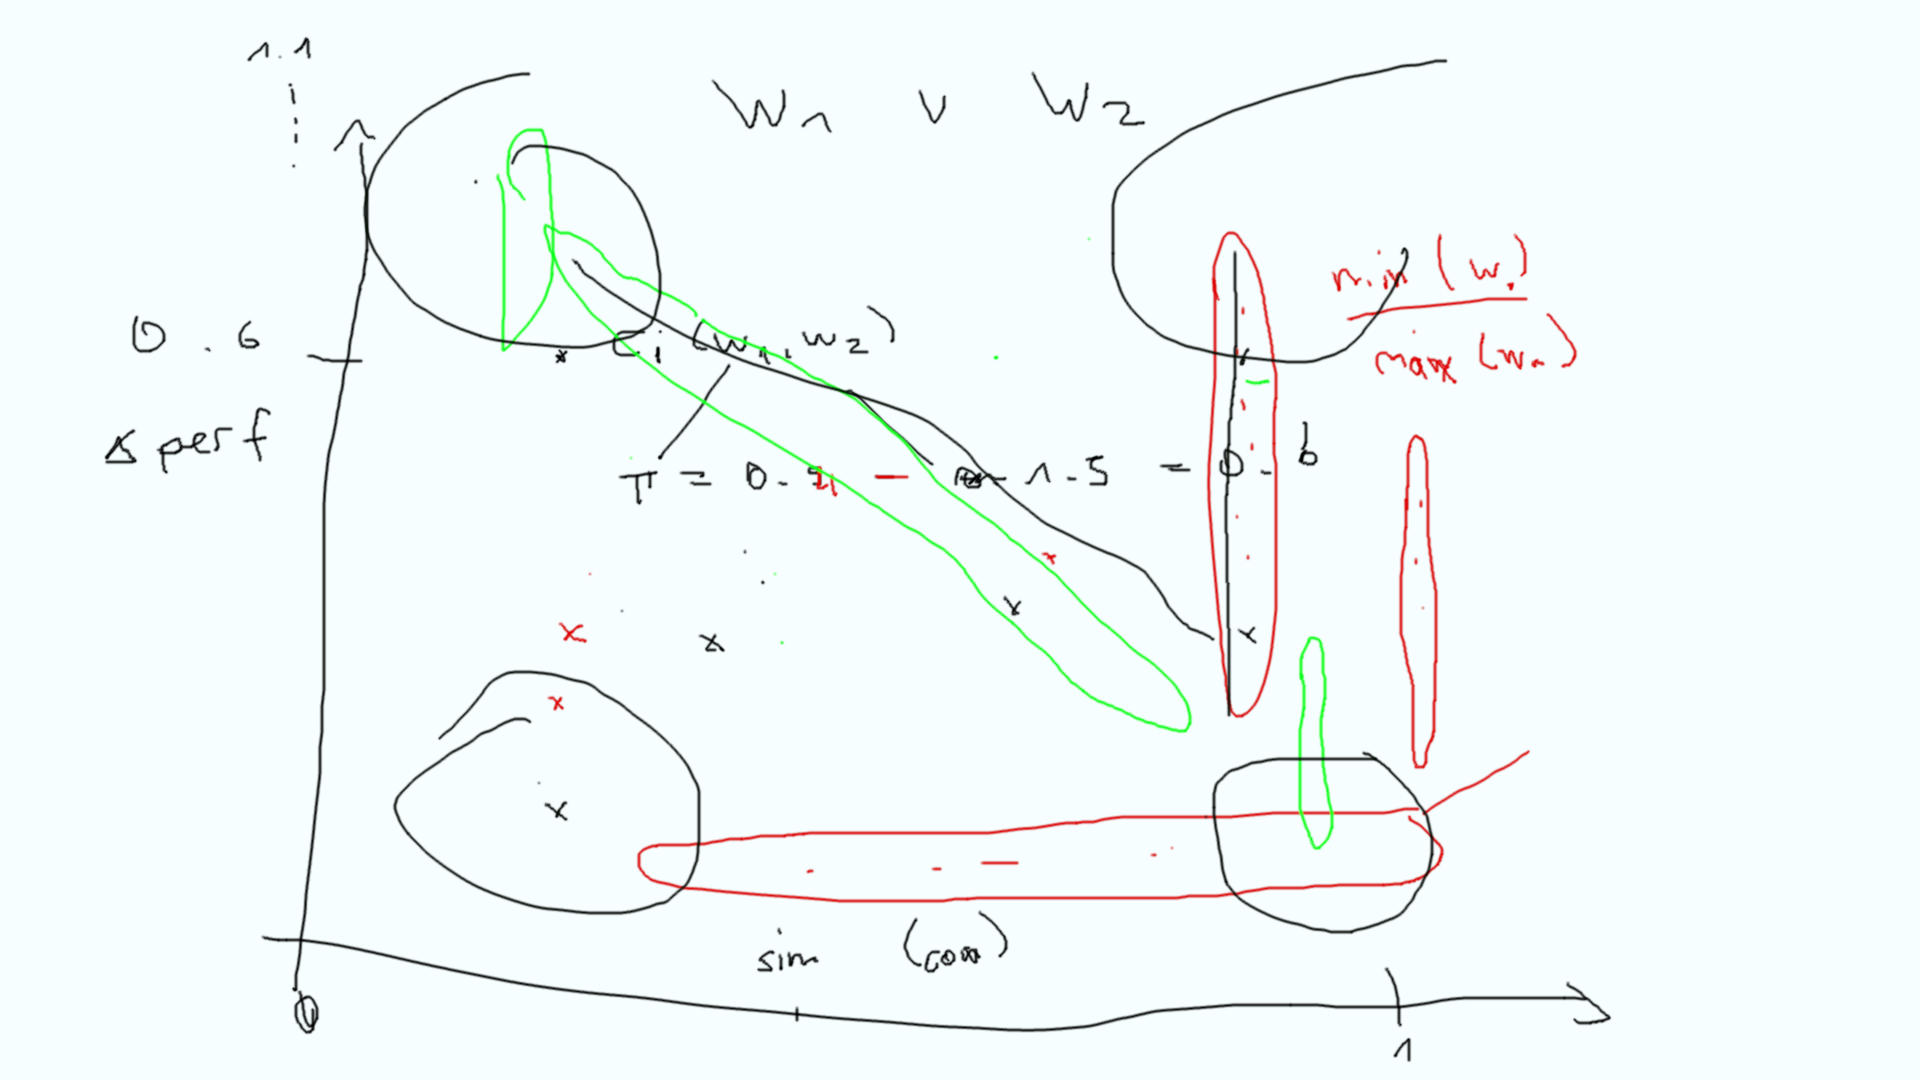
\includegraphics[width=\linewidth]{images/mockup.png}
		\caption{\batik}
	\end{subfigure}
	\begin{subfigure}{0.33\textwidth}
		\centering
		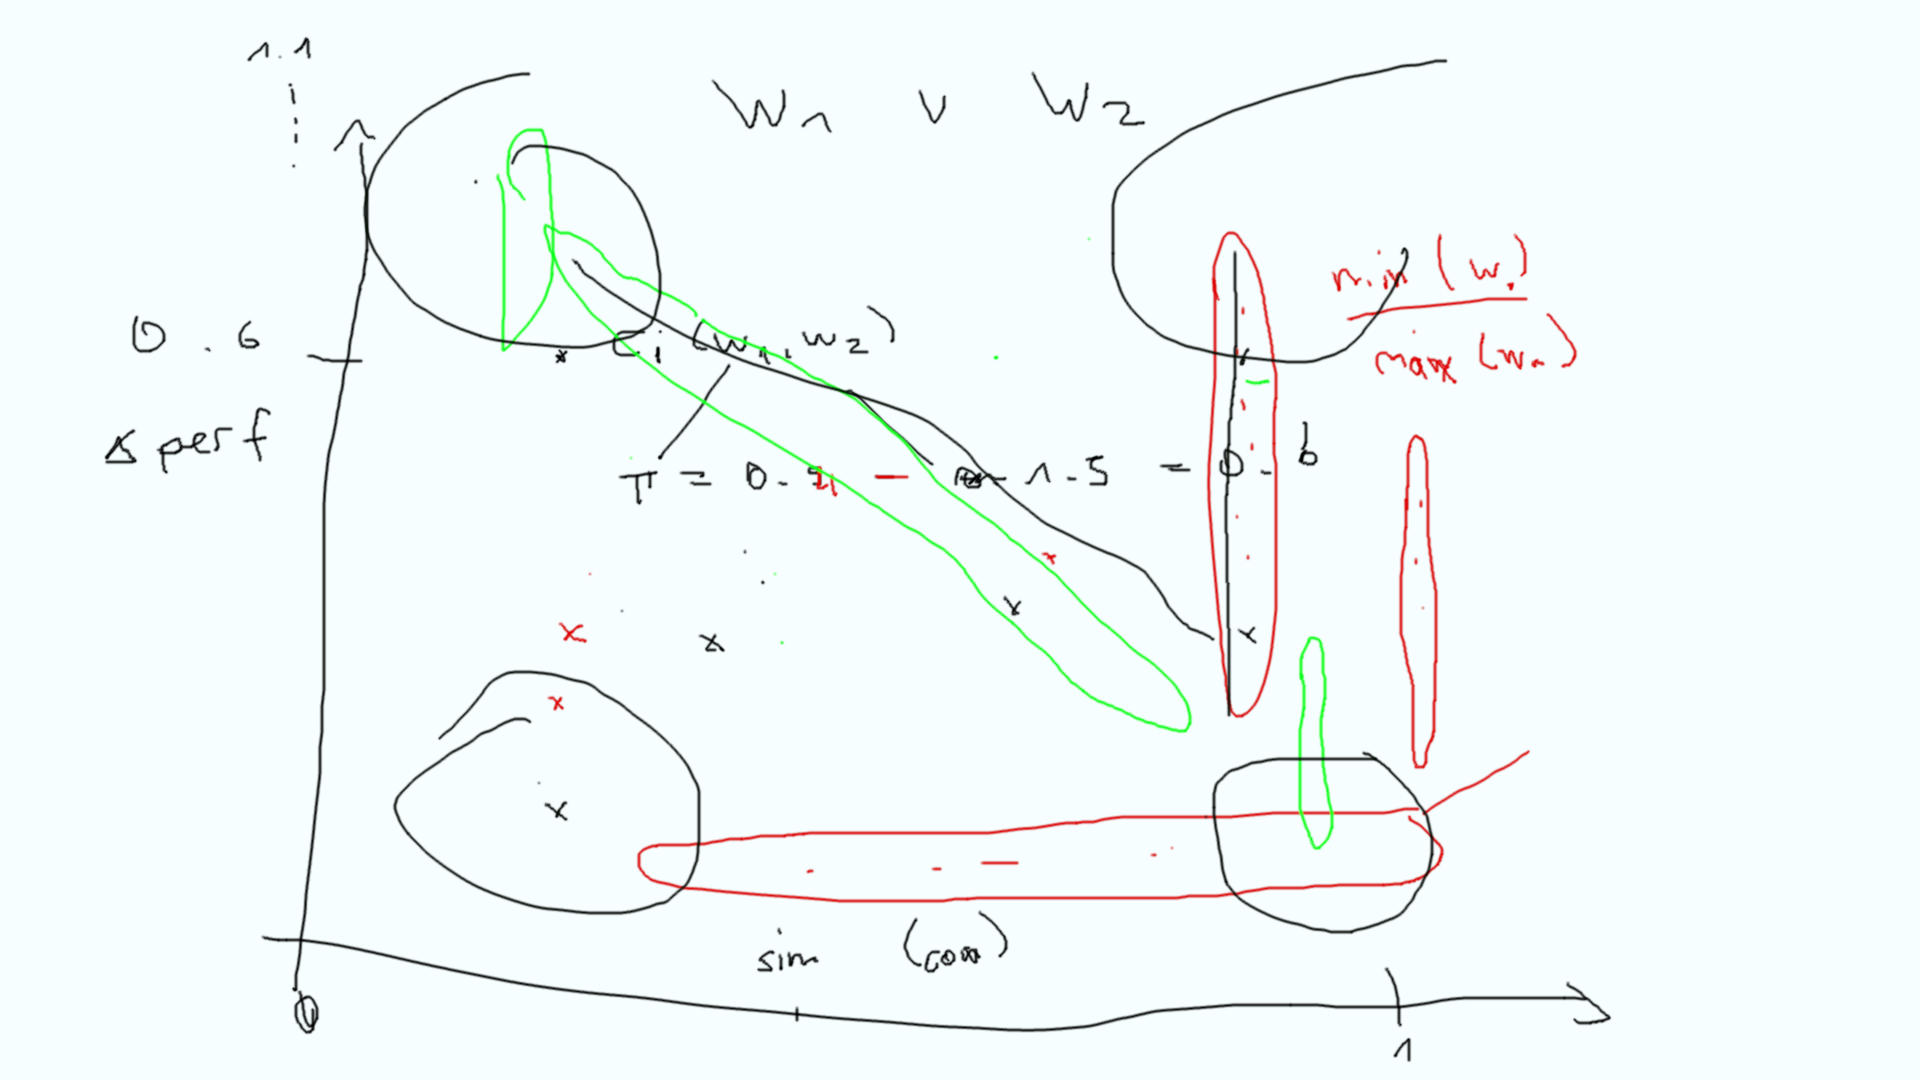
\includegraphics[width=\linewidth]{images/mockup.png}
		\caption{\dconvert}
	\end{subfigure}
	\begin{subfigure}{0.33\textwidth}
		\centering
		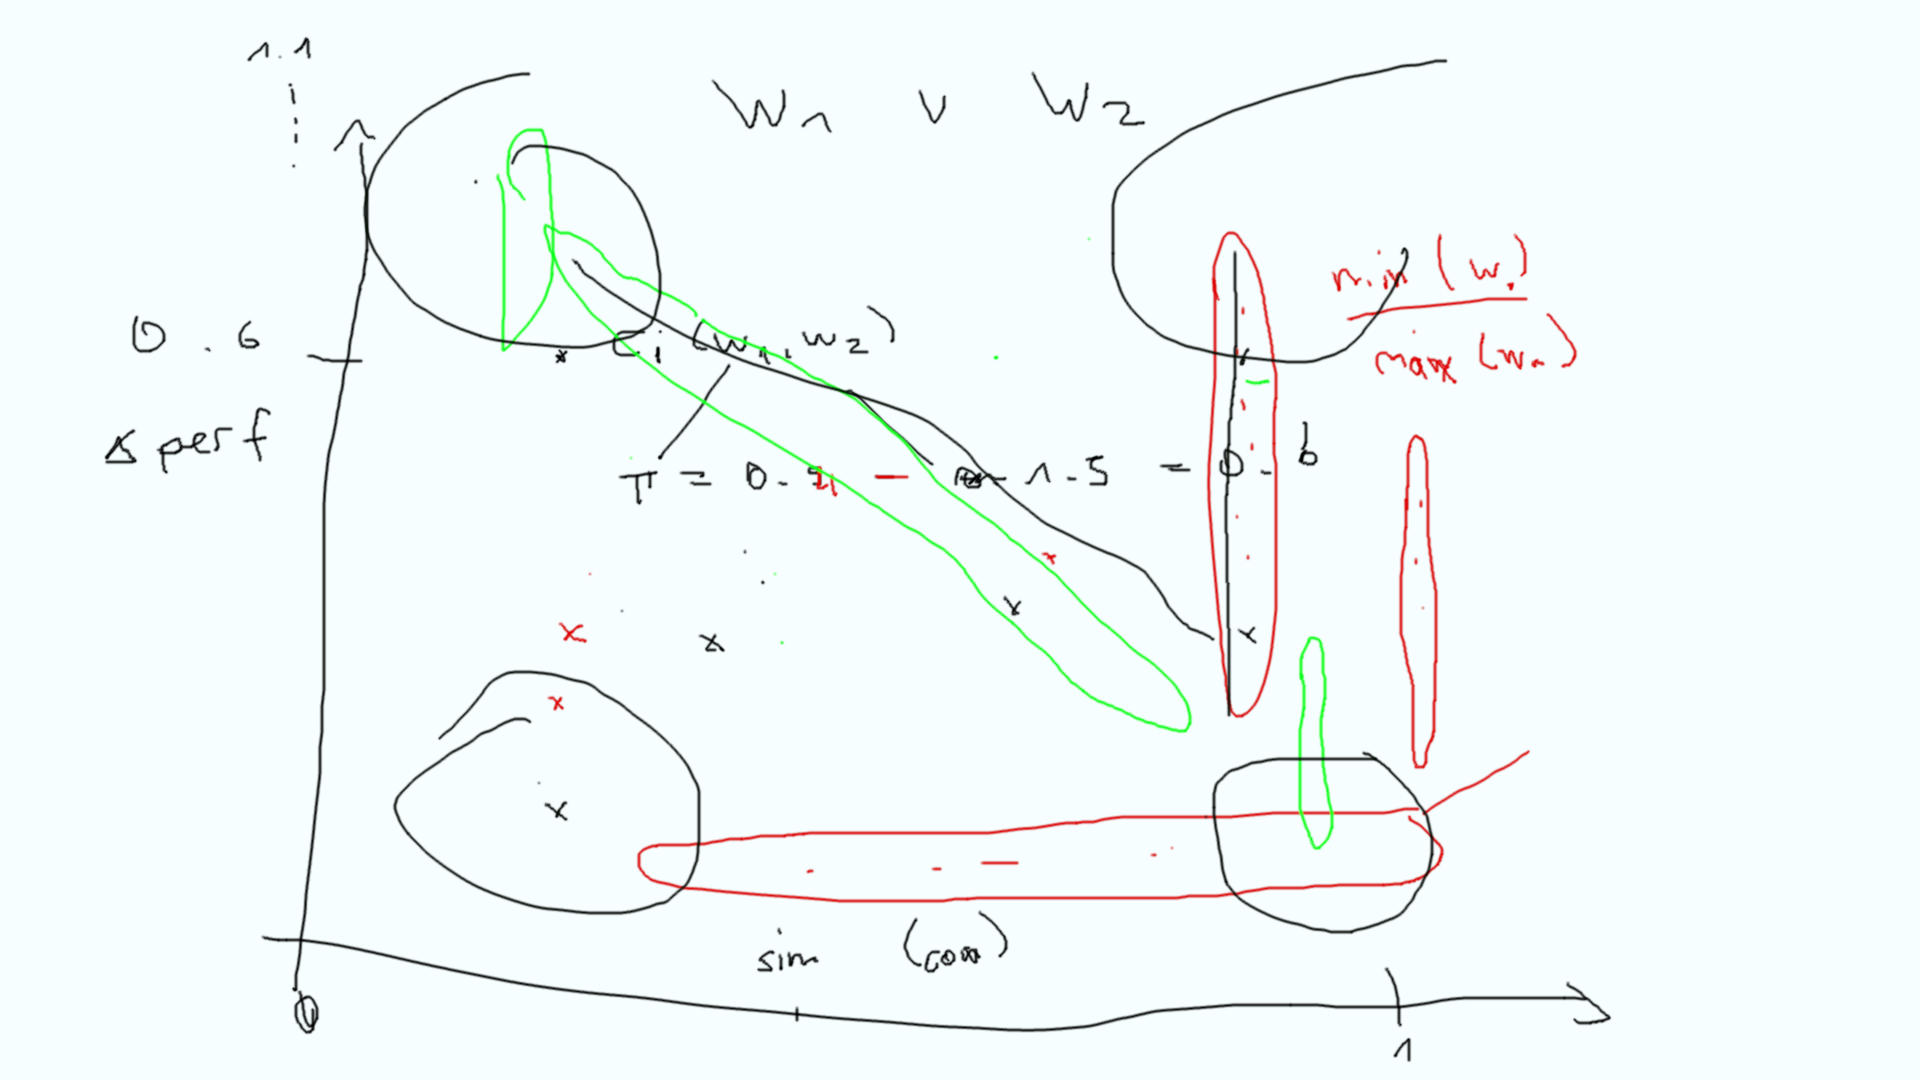
\includegraphics[width=\linewidth]{images/mockup.png}
		\caption{\htwo}
	\end{subfigure}
	\begin{subfigure}{0.33\textwidth}
		\centering
		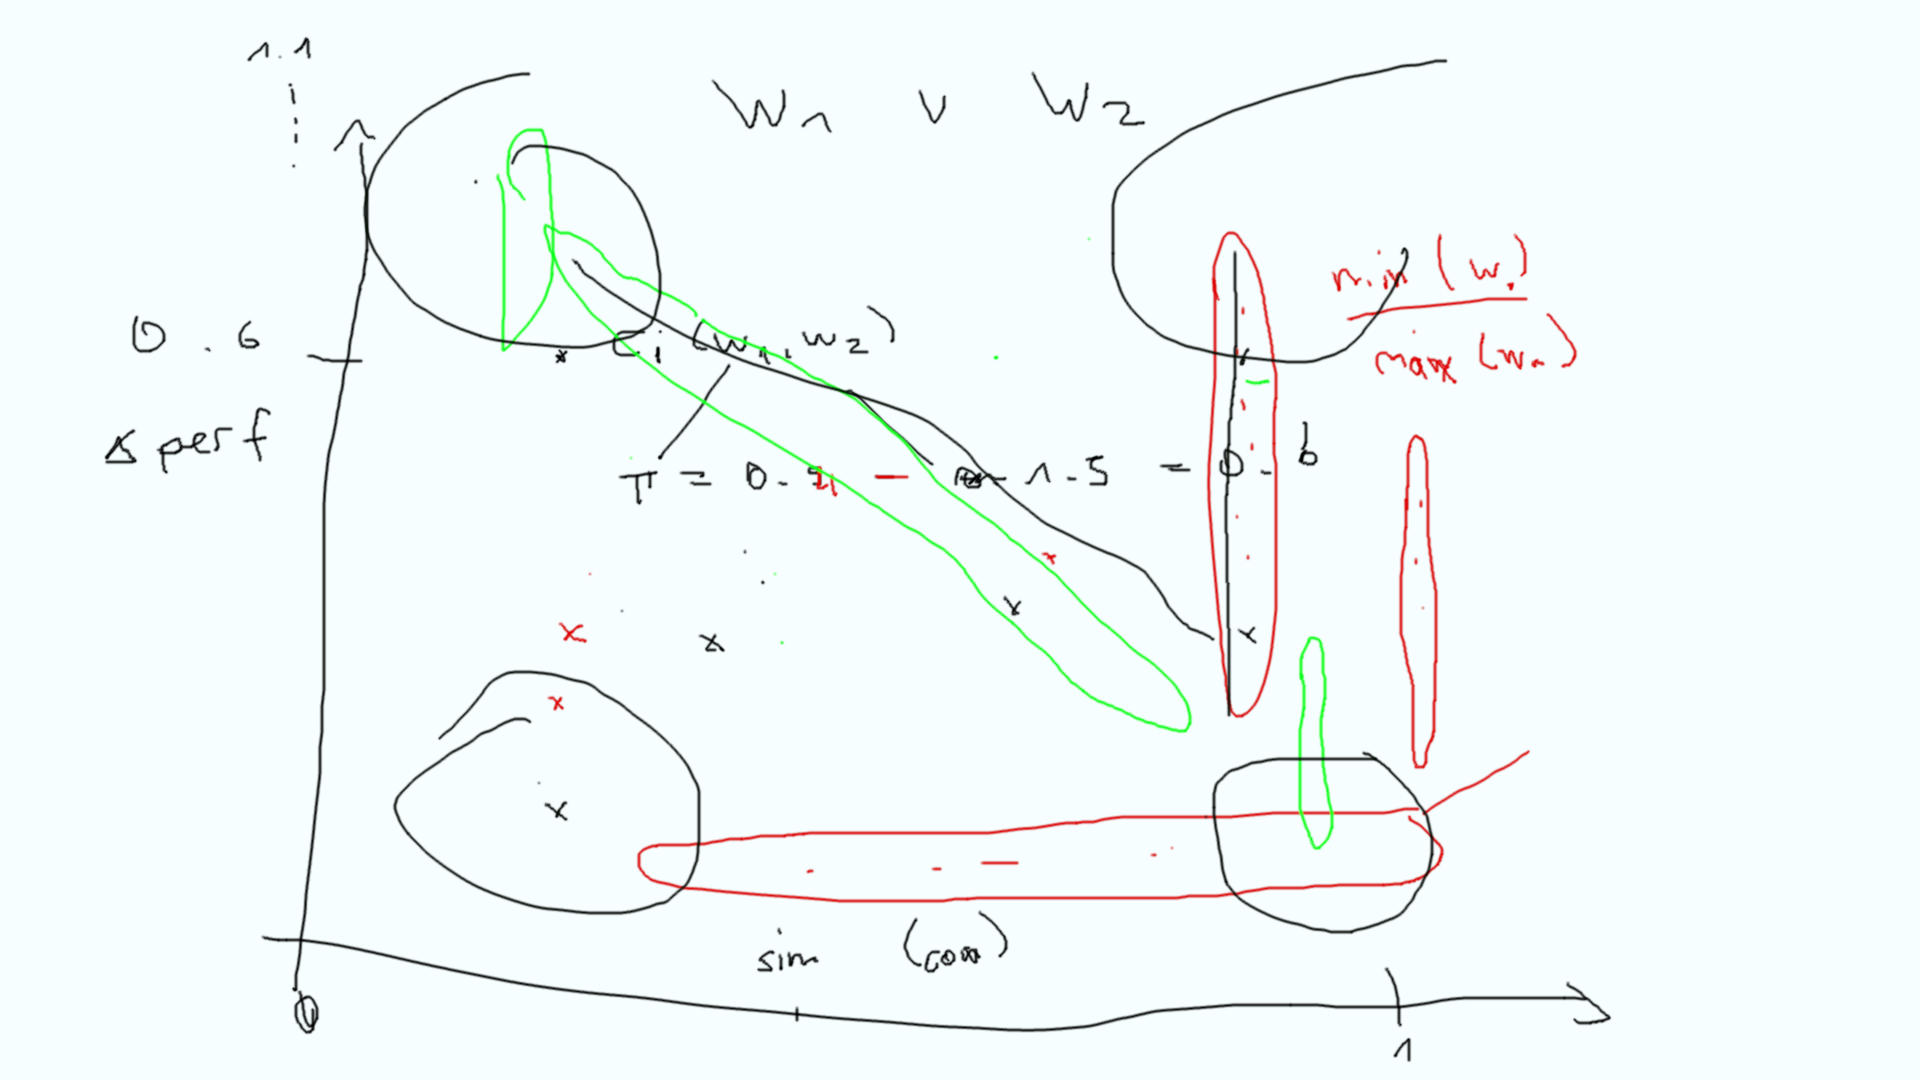
\includegraphics[width=\linewidth]{images/mockup.png}
		\caption{\jumper}
	\end{subfigure}
	\begin{subfigure}{0.33\textwidth}
		\centering
		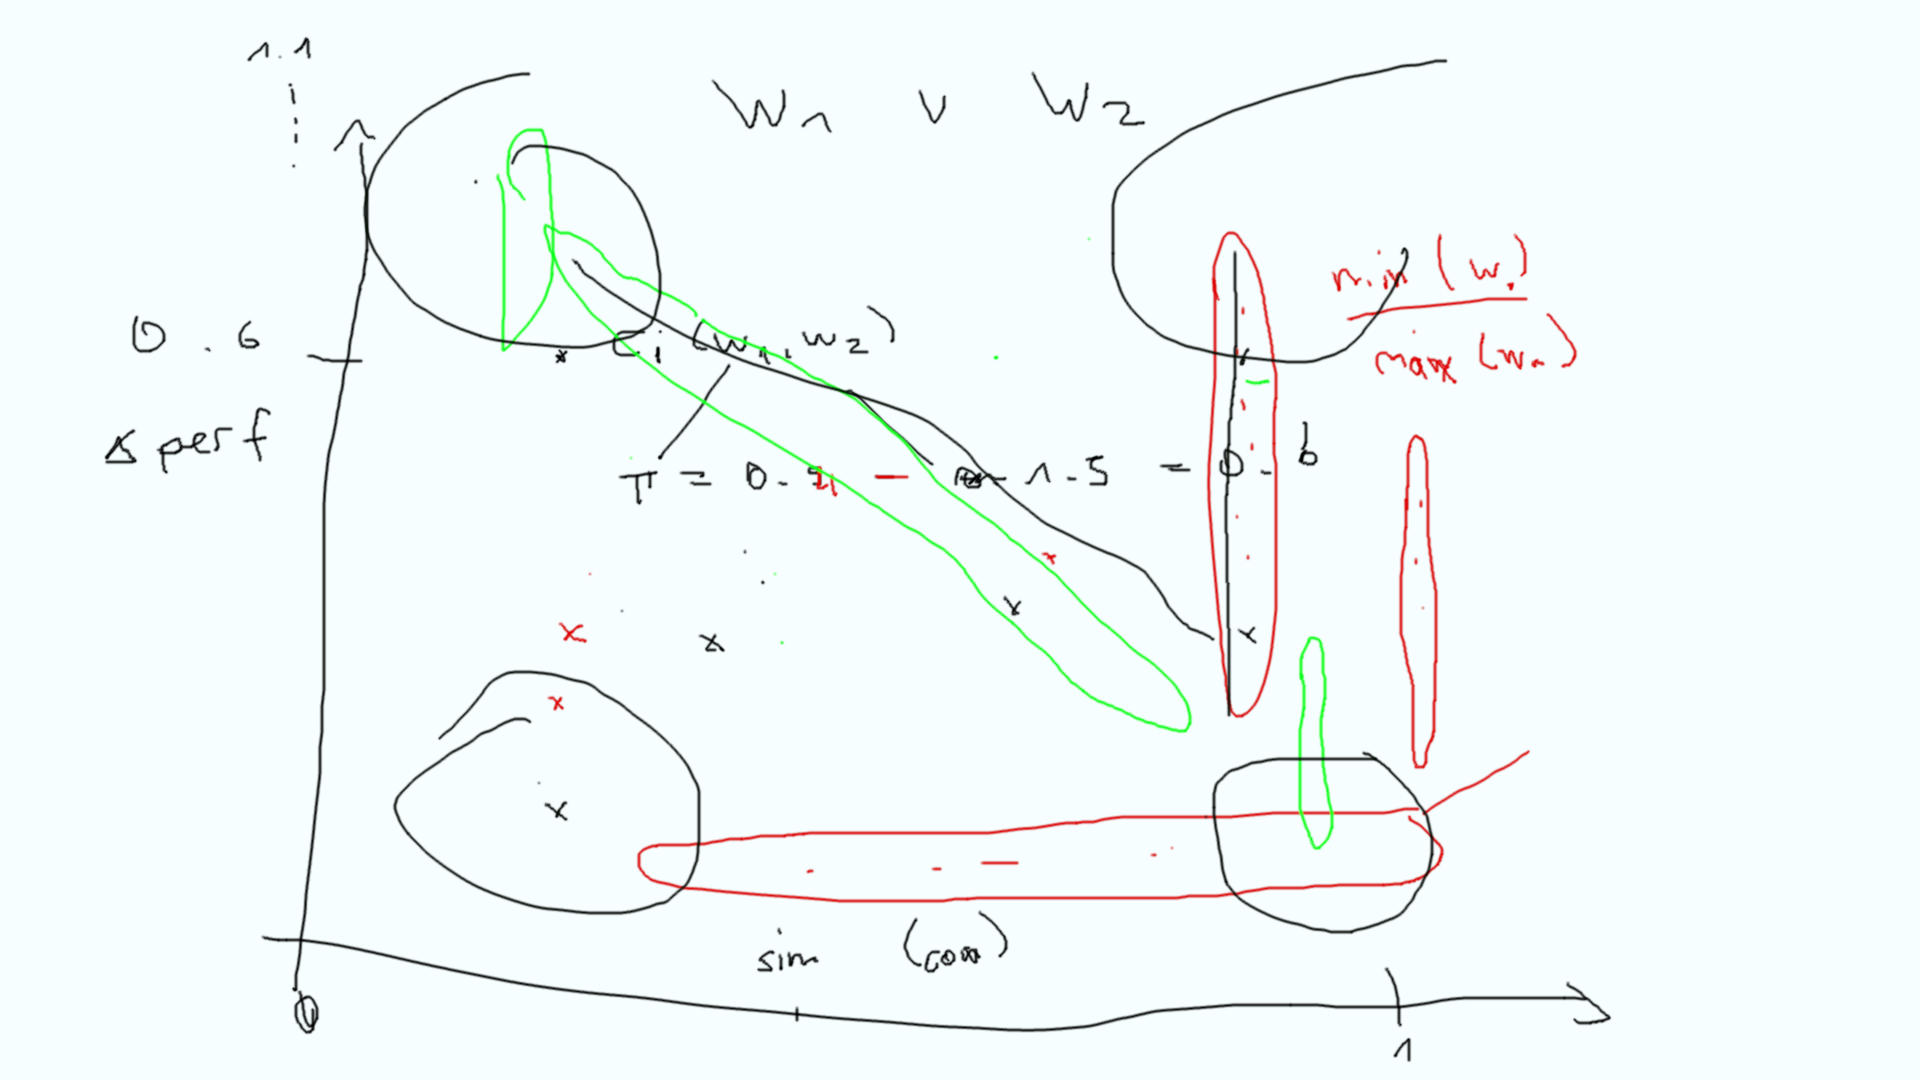
\includegraphics[width=\linewidth]{images/mockup.png}
		\caption{\jadx}
	\end{subfigure}
	\begin{subfigure}{0.33\textwidth}
		\centering
		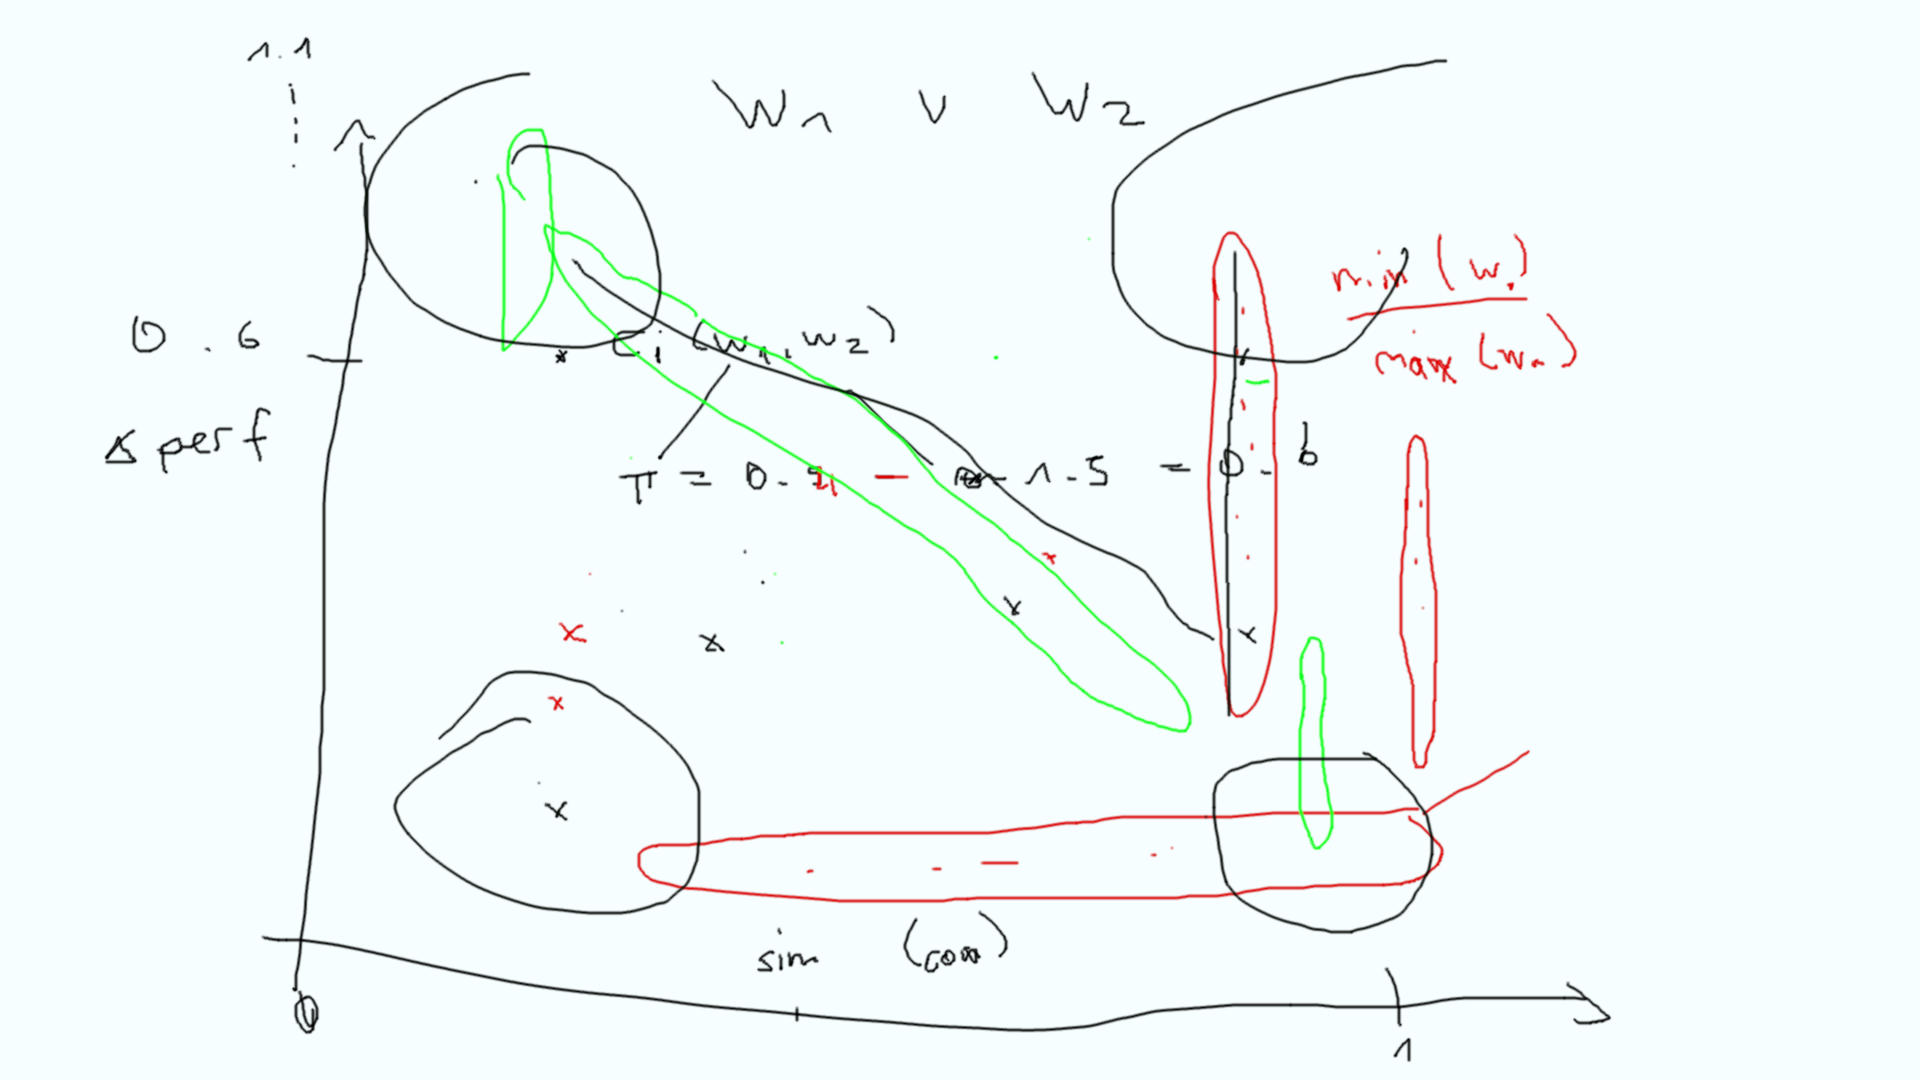
\includegraphics[width=\linewidth]{images/mockup.png}
		\caption{\kanzi}
	\end{subfigure}
	\caption{Relationship between differences in configuration code coverage and differences in relative configuration performance for pairs of workloads.}
	\label{fig:diff_config}
\end{figure*}

\subsubsection{Operationalization Across Options}


\section{Discussion}

\section{Threats to Validity}\label{sec:threats}
\paragraph{Internal Validity}\label{sec:internal_validity}

\begin{compactitem}
	\item dedicated hardware to mitigate measurement noise, 
	\item five repetitions per data point, 
	\item database experiments robustness assessed in pre-study,
	\item separate experiment runs for coverage analysis and performance measurement to avoid profiling averhead (assuming determinism)
	\item load generator overhead for databases, hence omitted memory consumption and other hardware-related performance indicators 
\end{compactitem}

\paragraph{External Validity}\label{sec:external_validity}
%A threat to generalizability is the selection of our subject systems since we only considered software written in Java. 
%While we deliberately opted for this class of subject systems for practical reasons, we address facet by selecting a large range of software systems and workloads from different application domains. 
%While one cannot generalize findings to other programming languages or environments without context, we are confident that domain-specific findings, such as for databases, may hold for further similar software systems.
\begin{compactitem}
	\item Java only, but different application domains,
	\item consistent with observations from related work
\end{compactitem}

\paragraph{Construct Validity}\label{sec:construct_validity}
\begin{compactitem}
	\item \textit{off-line instrumentation} vs. on-line instrumentation
	\begin{compactitem}
		\item avoid compiler optimizations or overhead from instrumented source code
		\item byte code ad-hoc instrumentation could increase overhead in a separate run
		\item byte-code instrumentation with Jacoco less precise than other techniques since mapping byte code instructions back to Java source code is not always trivial (observed before~\cite{luo_2019_cova})
	\end{compactitem}
	\item Coverage analysis for middle- to low-level languages face instrumentation bias
\end{compactitem}

\section{Conclusion}